%%%%%%%%%%%%%%%%%%%%%%%%%%%%%%%%%%%%%%%%%%%%%%%%%%%%%%%%%%%%%%%%%%%%%%%%%%%%%%%%
%2345678901234567890123456789012345678901234567890123456789012345678901234567890
%        1         2         3         4         5         6         7         8

\documentclass[letterpaper, 12 pt, conference]{ieeeconf}  % Comment this line out
                                                          % if you need a4paper
%\documentclass[a4paper, 12pt, conference]{ieeeconf}      % Use this line for a4
                                                          % paper

\IEEEoverridecommandlockouts                              % This command is only
                                                          % needed if you want to
                                                          % use the \thanks command
\overrideIEEEmargins
% See the \addtolength command later in the file to balance the column lengths
% on the last page of the document

\usepackage{hyperref}
\usepackage[utf8]{inputenc}
\usepackage{enumerate}
\usepackage{natbib}
\usepackage{graphicx}
\usepackage[spanish]{babel}
\hypersetup{
    colorlinks=true,
    linkcolor=blue,
    filecolor=magenta,      
    urlcolor=cyan,
}

% The following packages can be found on http:\\www.ctan.org
%\usepackage{graphics} % for pdf, bitmapped graphics files
%\usepackage{epsfig} % for postscript graphics files
%\usepackage{mathptmx} % assumes new font selection scheme installed
%\usepackage{times} % assumes new font selection scheme installed
%\usepackage{amsmath} % assumes amsmath package installed
%\usepackage{amssymb}  % assumes amsmath package installed

\title{\LARGE \bf
Práctica 2: teoremas de redes
}

%\author{ \parbox{3 in}{\centering Narshion Ngao*
%         \thanks{*Use the $\backslash$thanks command to put information here}\\
%         Msc. Computer Systems - 2018\\
%         Jomo Kenyatta University of Agriculture \& Technology \\
%       
%}}

\author{Universidad de San Carlos de Guatemala \\% <-this % stops a space
Escuela de Ciencias Físicas y Matemáticas\\
Laboratorio de Circuitos\\
Segundo Semestre 2019
}


\begin{document}



\maketitle
\thispagestyle{empty}
\pagestyle{empty}

\section{Objetivos}
\begin{itemize}
    \item General: Ejercitar el uso de teoremas de redes básicos para el cálculo de variables en circuitos resistivos.
    \item Específicos:
    \begin{enumerate}
    \item Comprobar la eficiencia de la Ley de Voltajes de Kirchhoff para análisis de corrientes y voltajes en mallas.
    \item Explorar el uso del Teorema de Thevenin para valores equivalentes en puntos específicos de interés en un circuito.
\end{enumerate}
\end{itemize}


\section{Materiales}
\begin{enumerate}
    \item 1 multímetro.
    \item 9 resistencias de cualquier valor 1/4W.
    \item 1 diodo rectificador de silicio.
    \item 1 potenciómetro de 1K ohm.
    \item Alambres para protoboard de cualquier tipo (y pinzas para cortarlo, si es necesario).
    \item 1 fuente.
    \item 1 protoboard.
    \item Opcional: computadora.
\end{enumerate}
\pagebreak

\section{Diagramas}

\begin{figure}[h!]
    \centering
    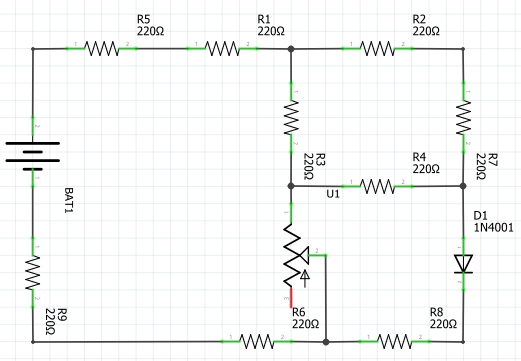
\includegraphics[scale=0.7]{C1.png}
    \caption{Esquema de circuito tres mallas.}
\end{figure}

\begin{figure}[h!]
    \centering
    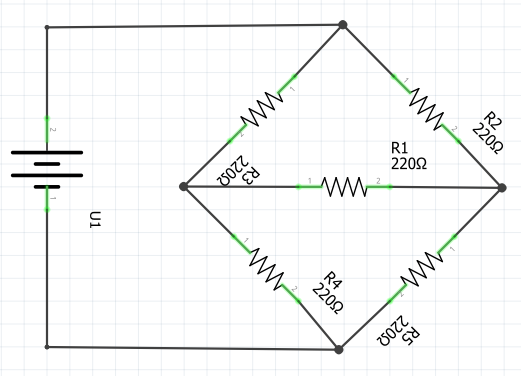
\includegraphics[scale=0.5]{C2.png}
    \caption{Esquema de puente de resistencias.}
\end{figure}


\section{Procedimiento y reporte de resultados}
Seguir todos los pasos que a continuación se enlistan respondiendo en una hoja adicional lo que sea requerido de forma ORDENADA y CLARA.

\begin{enumerate}
    \item Armar en un protoboard el circuito de la Figura 1.

\begin{figure}[h!]
    \centering
    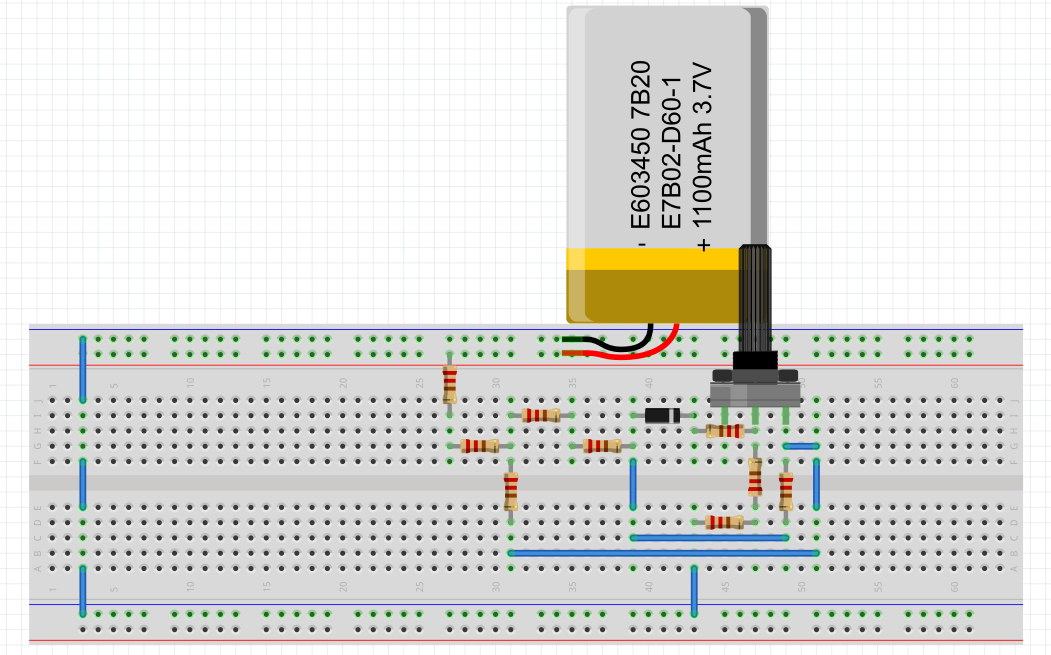
\includegraphics[scale=0.4]{B1.png}
    \caption{Circuito de Figura 1 en protoboard.}
\end{figure}

    \item Con los valores elegidos, calcular las ecuaciones de corrientes en la mallas en función del valor del potenciómetro.
    \item Llevar el potenciómetro a su máximo valor y medir:
    \begin{itemize}
        \item Corriente en R5.
        \item Corriente en R4.
        \item Voltaje en R8.
        \item Voltaje en R6.
    \end{itemize}
    \item Con las ecuaciones obtenidas en el inciso 2, obtener los valores teóricos (con valores ideales) para comparar con las mediciones del inciso 3.
    \item Realizar diagramas de incertezas para comparación de las cuatro mediciones.
    \item Armar en protoboard el puente de la Figura 2.
    
\begin{figure}[h!]
    \centering
    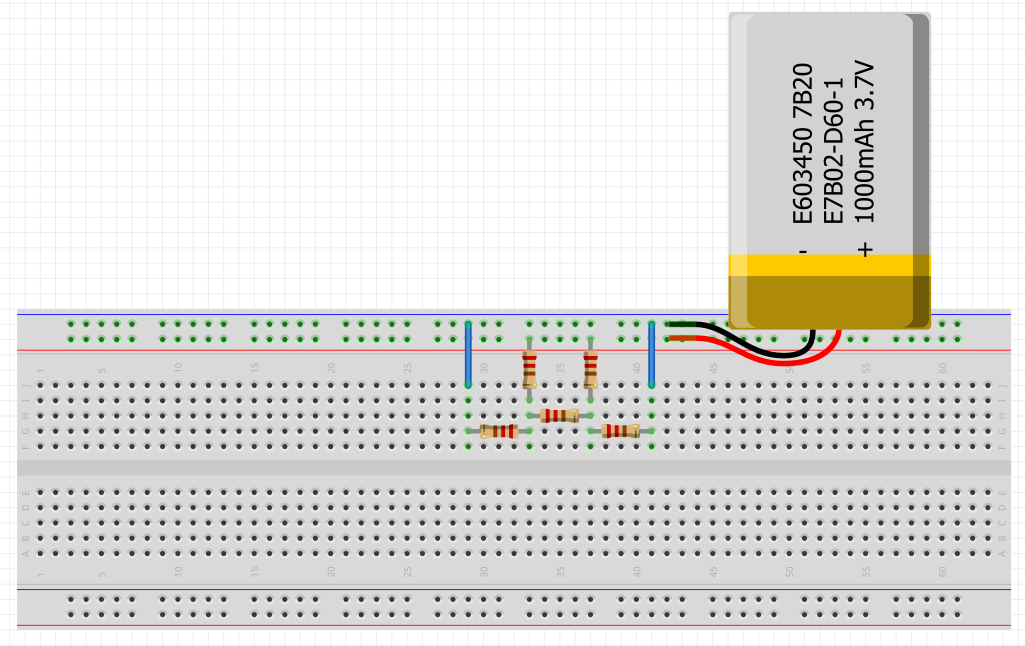
\includegraphics[scale=0.4]{B2.png}
    \caption{Circuito de Figura 2 en protoboard.}
\end{figure}
    
    \item Utilizando el teorema de Thevenin obtener la fuente y resistencia en serie total con la suposición de que R2 es la resistencia de carga que interesa analizar. Utilizar valores ideales y dejar constancia de todo el procedimiento. 
    \item Desconectar R2 del circuito. Con un multímetro, medir el voltaje en el lugar exacto en que se encontraba la resistencia.
    \item Apagar la fuente de voltaje del circuito.
    \item Medir la resistencia entre los dos puntos en que se encontraba R2.
    \item Medir R2 individualmente.
    \item Volver a concectar R2 en el circuito, encender la fuente y medir su caída de voltaje.
    \item Llenar la tabla a continuación y realizar diagramas de incertezas para los valores encontrados.
    \begin{table}[]
    \centering
\begin{tabular}{|c|l|l|}
\hline
\multicolumn{1}{|l|}{\textbf{}} & \textbf{Valor real} & \textbf{Valor ideal} \\ \hline
R2                              &                     &                      \\ \hline
Vth                             &                     &                      \\ \hline
Rth                             &                     &                      \\ \hline
Vr2                             &                     &                      \\ \hline
\end{tabular}
\end{table}
    \item Escribir las conclusiones de la práctica.
\end{enumerate}
\addtolength{\textheight}{-12cm}   % This command serves to balance the column lengths
                                  % on the last page of the document manually. It shortens
                                  % the textheight of the last page by a suitable amount.
                                  % This command does not take effect until the next page
                                  % so it should come on the page before the last. Make
                                  % sure that you do not shorten the textheight too much.

\end{document}